%------------------------------------------------------------------------------

\chapter{Θεωρία}
\label{chapter3} 

Το κεφάλαιο αυτό θα αναλύσει ότι χρειάζεται να ξέρει ο αναγνώστης για να
κατανοήσει το κεφάλαιο της υλοποίησης. Αρχικά θα περιγράψουμε εκτενέστερα την
διαδικασία που ακολουθείται στο σύστημα RPython για την μεταγλώττιση (π.χ. του
PyPy), έτσι ώστε να ξέρει ο αναγνώστης σε ποιο "χρονικό" σημείο θα λάβει χώρα το
εγχείρημά μας. Έπειτα θα παραθέσουμε με λεπτομέρεια την θεωρία της μεθόδου που
θα υλοποιήσουμε.

%------------------------------------------------------------------------------

\section{Διαδικασία Μεταγλώττισης στο σύστημα RPython}

\subsection{Επισκόπηση}

Ο σκοπός του συστήματος και του \textit{toolchain} του RPython είναι να
μεταφράσει προγράμματα (κυρίως μεταφραστές) γραμμένα σε RPython με
αποτελεσματικότητα ανεξάρτητα με το ποια πλατφόρμα είναι το target του. Το
default target είναι το \textit{C backend} (παραγωγός κώδικα C) και σε αυτό θα
αναφερόμαστε όταν δίνουμε παραδείγματα.

Το σύστημα στην πραγματικότητα δεν βλέπει ποτέ κανονικό κώδικα Python ή
δέντρα, αλλά ξεκινά με \textit{αντικείμενα κώδικα} (code objects) βασισμένα
στις συναρτήσεις που έχουν δοθεί ως είσοδος και τα μετατρέπει με
\textit{abstract interpretation}\cite{CousotCousot77}\cite{debray1995abstract}
σε γραφήματα ροής. Η βασική δηλαδή δομή δεδομένων (unit), πάνω στην οποία
δουλεύει το σύστημα επομένως, είναι τα γραφήματα ροής (σε SSA\cite{ssa} form)
βασισμένα σε function code objects. Ένα γράφημα για κάθε συνάρτηση. Αυτά τα
γραφήματα είναι απλώς ένας ακόμα τρόπος αναπαράστασης του προγράματος, αλλά
πιο κατάλληλος για "αφαιρετικές" εργασίες μεταγλώττισης και βελτιστοποίσης
(π.χ. εξαγωγή τύπων\footnote{βλ. type inference}).

Η διαδικασία είναι οργανωμένη σε στάδια (βλ. Σχήμα \ref{figure-1}).

\begin{enumerate}

\item \textbf{Import \& Flow Analysis}: Εδώ ο αρχικός κώδικας φορτώνεται στην
μνήμη και υφίσταται τις βασικές διαδικασίες συντακικής ανάλυσης. Μετατρέπεται
αρχικά σε tokens, έπειτα σε μια ενδιάμεση μορφή (Python bytecode) – όπως σε
όλους τους μεταγλωττιστές – και τέλος στα διαγράμματα ροής του PyPy. Από αυτό
το στάδιο και έπειτα φυσικά βρίσκεται μόνο μέσα στην τοπική μνήμη, σε μια 
αρκετά "στατική" μορφή για τα δεδομένα του RPython.

\item \textbf{Annotator subsystem}: Εδώ ενεργοποιούνται οι περισσότερο
αφαιρετικές μέθοδοι ερμηνείας του κώδικα. Μια καθολική ανάλυση, που θα 
ξεκινήσει από το σημείο εισόδου του κάθε διαγράματος (entry point), θα "εξάγει"
γενικές πληροφορίες για τον κώδικα και θα συμπεράνει τους τύπους που μπορεί η 
κάθε μεταβλητή να φιλοξενήσει κατά το runtime βάσει φυσικά των συμφραζομένων.
Μετά από αυτό το βήμα, έχουμε annotated flow graphs.

\item \textbf{RTyper}: Αυτό το σύστημα χρησιμοποιεί τους
\textit{υποσημειώμένους} είδικούς προσωρινούς τύπους που έχει προσθέσει ο
annotator για να μετατρέψει τα statements και τις εντολές στα γραφήματα σε
εντολές χαμηλότερου επιπέδου. Είναι ουσιαστικά μια γέφυρα μεταξύ των γραφημάτων
και των παραγωγών κώδικα.

\item \textbf{Optimizations}: Η βελτιστοποίηση στο PyPy γίνεται εδώ. Το project
περιλαμβάνει – και εφαρμόζει –  μια πληθώρα βελτιστοποιήσεων, όπως αυτά που
αναφέραμε στο κεφάλαιο \ref{chapter2}. Επίσης το δικό μας module θα λάβει χώρα
εδώ.

\item \textbf{Προετοιμασία Γραφημάτων}: Εδώ γίνονται οι τελικές ενέργειες πριν
την παραγωγή κώδικα. Τα γραφήματα εδώ λ.χ. υφίσταντο ανάλυση για τον υπολογισμό
ονομάτων μεταβλητών (για λόγους όπως debugging) κ.α. Σημαντικότερες όμως είναι
οι εξής ενέργειες:

\begin{itemize}

\item \textbf{Exception transformer}: Ο "μετατροπέας εξαιρέσεων" ενεργοποιείται
σε αυτό το σημείο και θα εισάγει τον απαραίτητο κώδικα για τη διαχείριση των
εξαιρέσεων που τυχαίνει να υπάρχουν.

\item \textbf{Garbage Collection Transformer}: Εδώ παίρνει σειρά το ειδικό
εργαλείο διαχείρισης "σκουπιδιών μνήμης". Αυτό εκτελεί όποιες ενέργειες
χρειάζονται για την σωστή διαχείριση μνήμης. Αφού η Python είναι πλήρως 
δυναμική γλώσσα και δεν απαιτεί από τον προγραμματιστή να διαχειρίζεται την 
μνήμη που χρειάζεται μόνος του, είναι απαραίτητη η ύπαρξη ενός υποσυστήματος
διαχείρισης σκουπιδιών μνήμης.

\end{itemize}

\item \textbf{Code Generation}: Εδώ τα ήδη μαρκαρισμένα, σημειωμένα,
βελτιστοποιημένα γραφήματα θα μετατραπούν σε κώδικα μηχανής. Εδώ υπάρχουν 
πολλοί "γεννήτορες" κώδικα ανάλογα με τις ανάγκες. Ο βασικότερος και ο πιο 
σημαντικός είναι ο παραγωγός κώδικα C. Αρχικά, τα γραφήματα θα μετατραπούν σε 
άλλα αντίστοιχα, ανάλογα με τον γεννήτορα και έπειτα αυτά θα μετατραπούν σε
κώδικα ανάλογα με την επιλογή (π.χ σε κώδικα C)

\item Τέλος ο κώδικας αυτός θα οδηγηθεί στον μεταφραστή της εκάστοτε επιλογής
(π.χ. \texttt{gcc}) για να παραχθεί το εκτελέσιμο αρχείο.

\end{enumerate}

\begin{figure}[h]
\centering
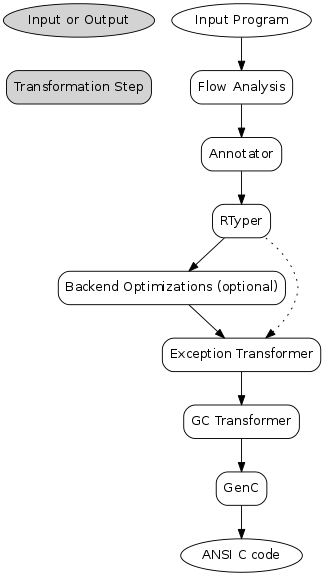
\includegraphics[width=0.5\textwidth]{diagram.png}
\caption{diagram of RPython translation process}
\label{figure-1}
\end{figure}

\subsection{Γραφήματα Ροής}

\subsubsection{Τρόπος δημιουργίας}

Ο σκοπός του κατασκευαστή γραφημάτων (υλοποιημένος στο module
\texttt{rpython.flowspace}) είναι να μετατρέψει τα αντικείμενα συναρτήσεων σε
γραφήματα. Κανονικά οι μεταγλωττιστές παίρνουν μια συνάρτηση και την
μετατρέπουν σε ενδιάμεσο bytecode κώδικα σε κάποια εικονική μηχανή (VM) και
έπειτα την τρέχουν. Στο RPython όμως χρησιμοποιείται ένα \textit{abstract
interpretation} το οποίο λειτουργώντας αφαιρετικά μετατρέπει τον ενδιάμεσο
κώδικα στα βασικα \texttt{Block}, τα οποία περιέχουν όλες τις εντολές οι
οποίες επιδρούν πάνω σε αντικείμενα Python. Το αποτέλεσμα της κάθε εντολής
αποθηκεύεται προσωρινά σε μια μεταβλητή η οποία μπορεί να χρησιμοποιηθεί στις
επόμενες. Για ένα παράδειγμα βλ. Σχήμα \ref{figure-2} το οποίο είναι ένα
γράφημα μιας απλής συνάρτησης με ένα if branch. Φαίνεται η γενική εικόνα των
γραφημάτων, το branch καθώς ο τρόπος που επαναχρησιμοποιούνται οι προσωρινές
μεταβλητές αποτελεσμάτων ανάλογα με τις ανάγκες.

\begin{figure}[h]
\centering
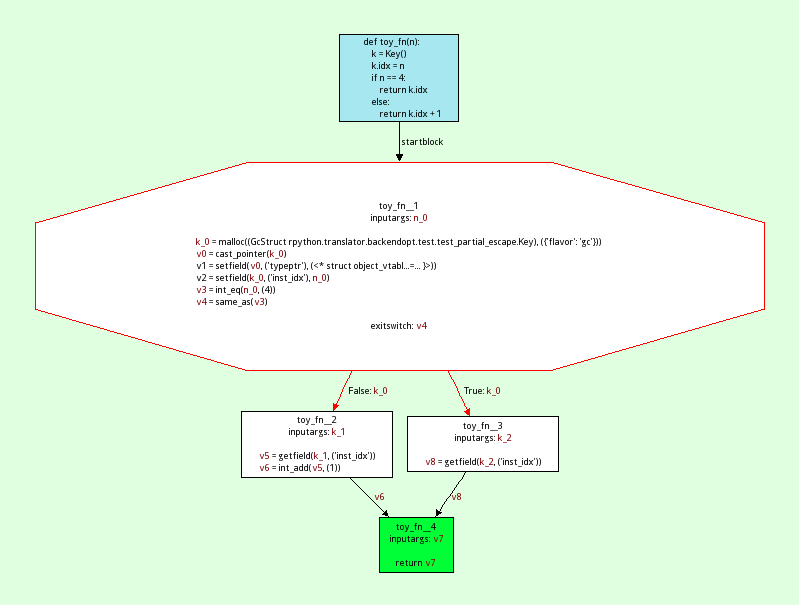
\includegraphics[width=\textwidth]{simple-func-bef.png}
\caption{simple function flow diagram}
\label{figure-2}
\end{figure}

Ο κατασκευαστής "κλείνει" ένα \texttt{Block} και πάει στο επόμενο σε 2 
περιπτώσεις:

\begin{enumerate}

\item Περίπτωση κλήσης \texttt{is\_true()}. Όταν συμβαίνει αυτό, ο \textit{
abstract interpreter} δεν ξέρει φυσικά αν η συνθήκη θα είναι \textit{True} ή
\textit{False} - αφού η γλώσσα μας είναι δυναμική – οπότε θα πρέπει να τις 
ακολουθήσει και τις 2, δημιουργώντας αντίστοιχα άλλες ροές (δηλαδή
\texttt{Blocks}) για την κάθεμια.

\item Περίπτωση εμφάνισης \textit{joinpoint}. Αυτή η περίπτωση λαμβάνει χώρα
όταν η επόμενη εντολή, που πρόκειται να καταγράψουμε στο τρέχον \texttt{Block},
έχει ήδη καταγραφεί ή καταγράφεται τώρα από άλλο \texttt{Block}. Αυτό σημαίνει
ότι ο μεταγλωττιστής έχει κλείσει κάποιον βρόγχο και πρόκειται να μεταγλωττίσει
κώδικα τον οποίο έχει ήδη "δει". Τότε ο μεταγλωττιστής σταματά, και
δημιουργείται ένα \texttt{Link} απο το τρέχον \texttt{Block} στο προηγούμενο,
έτσι ώστε να κλείσει ο βρόγχος και στο διάγραμμα και να υπάρχει πιστή
αναπαράσταση του κώδικα.

\end{enumerate}

\subsubsection{Το μοντέλο}

Η βασική συνάρτηση που δημιουργεί τις δομές δεδομένων που απαρτίζουν το μοντέλο
είναι η \texttt{build\_flow()}. Η μονάδα (unit) ροής είναι το αντικείμενο
\texttt{FunctionGraph} το οποίο μαζί με τα υπόλοιπα (που συνήθως περιέχονται σε
αυτό) ορίζονται στο αρχείο \texttt{rpython/flowspace/model.py}. Τα περιγράφουμε
παρακάτω:

\begin{itemize}

\item \texttt{FunctionGraph} Το διάγραμμα ροής μια συνάρτησης. Είναι η βασική
δομή δεδομένων του μεταγλωττιστή. Περιέχει αναφορές και μια λίστα απο
\texttt{Blocks}, τα οποία συνδέονται με \texttt{Links}. Βασικά κομμάτια του
είναι:

\begin{enumerate}
\item \textbf{startblock:} Το πρώτο block του γραφήματος. Είναι το σημείο
εισόδου για την ροή του προγράμματος όταν αυτή φτάσει σε αυτή την συνάρτηση. Οι
παράμετροι εισόδου θα δοθούν σε αυτό το block. Αυτό το block θα δείχνει όπως
και όλα τα άλλα σε επόμενα ανάλογα με την ροή.
\item \textbf{returnblock:} Το μοναδικό block στο κάθε γράφημα που μπορεί να
εκτελέσει μια "επιστροφή" της συνάρτησης στην ροή του ανώτερου επίπεδου
(function return). Είναι πάντα άδειο και δεν περιέχει ούτε την εντολής
επιστροφής – αυτή υπονοείται. Τα links δείχνουν εδώ όταν και μόνο όταν θέλουν
να τερματίσουν την συνάρτηση. Η μοναδική παράμετρος είναι η τιμή επιστροφής.
\item \textbf{exceptblock:} Αυτό και το παραπάνω είναι τα μόνα blocks που
μπορούν να τερματίσουν την ροή. Είναι το μοναδικό block που μπορεί να
"πυροδοτήσει" μια εξαίρεση. Δέχεται 2 τιμές· η πρώτη είναι η κλάση της εξαίρεσης
και η δεύτερη η τιμής της. Η μόνη περίπτωση να υπάρχει link προς αυτό το block
είναι η ρητή πυροδότηση εξαίρεσης από το πρόγραμμα.
\end{enumerate}

\item \texttt{Block} Το πιο σημαντικό κομμάτι ενός γραφήματος. Ένα γράφημα
ουσιαστικά είναι μια λίστα από blocks. Ένα block περιέχει μια λίστα από
\texttt{SpaceOperation}s, δηλαδή μια λίστα από εντολές. Λεπτομερειακά
αποτελείται από:

\begin{enumerate}
\item \textbf{inputargs:} Είναι μια λίστα με όλες τις μεταβλητές (με καινούργια
ονόματα) που μπορούν να εισέλθουν στο block από οποιοδήποτε προηγούμενο. Η
αντιστοίχηση των παλιών ονομάτων που υπάρχουν στα links με τα καινούργια 
γίνεται ένα προς ένα (π.χ. η πρώτη στα link με την πρώτη στη λίστα).
\item \textbf{operations:} Η λίστα με τις εντολές που θα τρέξουν όταν η ροή
καταλήξει σε αυτό το block. Θα τρέξουν όλες σειριακά χωρίς εξαιρέσεις. Οι
εντολές υποδεικνύονται από \texttt{SpaceOperation}s (βλ. πιο κάτω).
\item \textbf{exits:} Λίστα με πιθανά \textit{άλματα} (jumps). Φυσικά περιέχει
links. Σε "συνεργασία" με το επόμενο μέλος καθορίζει που θα προχωρήσει η ροή 
του προγράμματος. Φυσικά περιέχει ένα ή περισσότερα links.
\item \textbf{exitswitch:} Τα περιεχόμενα αυτού του μέλους ποικίλλουν:

\begin{enumerate}
\item Δεν υπάρχει \textit{jump} και περιέχει \texttt{None}. Το \textit{exits}
περιέχει ένα link.
\item Άλμα υπό συνθήκη. Σε αυτή την περίπτωση το \textit{exitswitch} είναι μια
από τις μεταβλητές του block. Σε συνεργασία με ένα αντίστοιχο
\textit{exitcase} στα \texttt{Link}s, διευθετεί τις περιπτώσεις των branches.
Η ροή θα ακολουθήσει το \texttt{Link}, του οποίου το \textit{exitcase},
ταιριάζει με το \textit{exitswitch} του \texttt{Block}. Αν δεν υπάρχει 
ταίριασμα τότε έχουμε runtime error.
\item Εξαίρεση. Το \textit{exitswitch} περιέχει
\texttt{Constant(last\_exception)}. Το πρώτο \texttt{Link} του \textit{exits}
περιέχει \texttt{None} στο \textit{exitcase} του για την περίπτωση που δεν
υπάρχει εξαίρεση. Τα υπόλοιπα links δείχνουν στα διάφορα classes των εξαιρέσεων
και ακολουθούνται αντίστοιχα. Φυσικά με αυτόν τον τρόπο "προστατεύτεται" μόνο η
τελευταία εντολή.
\item Επιστροφή. Περίπτωση \textit{Returnblock}. Το \textit{exitswitch}
και το \textit{operations} είναι άδεια και το \textit{exits} είναι ρυθμισμένο 
σε \texttt{None}.
\end{enumerate}

\end{enumerate}

\item \texttt{Link} Αποτελεί την σύνδεση μεταξύ των Blocks. Περιέχει:

\begin{enumerate}
\item \textbf{prevblock:} Το προηγούμενο \texttt{Block} από το οποίο δείχνει 
αυτό το \texttt{Link}.
\item \textbf{target:} Το \texttt{Block} στο οποίο δείχνει. Μπορεί να είναι 
μόνο ένα. Αν το \texttt{Block} πρέπει να δείξει σε περισσότερα, τότε πρέπει να 
υπάρχουν πολλά \texttt{Link}s.
\item \textbf{args:} Λίστα με \texttt{Variable}s και \texttt{Constant}s. Βλ. 
παραπάνω.
\item \textbf{exitcase:} Βλ. παραπάνω.
\item \textbf{last\_exception:} Εδώ θα τοποθετηθεί (στο runtime) η κλάση 
εξαίρεσης σε τέτοια περίπτωση, αν το \texttt{Link} δείχνει σε \texttt{Block} 
εξαιρέσεων.
\item \textbf{last\_exc\_value:} Ομοίως εδώ θα τοποθετηθεί η τιμή.
\end{enumerate}

\item \texttt{SpaceOperation} Υποδεικνύει μια "εντολή". Είτε καταγεγραμμένη 
είτε δημιουργημένη από τον ίδιο τον μεταφραστή. Σε αυτό το σημείο οι εντολές 
είναι σχετικά περιορισμένες (λ.χ. δεν μπορούν να πυροδοτήσουν μια εξαίρεση).
Αυτό σημαίνει ότι ο μεταφραστής μπορεί να υποθέσει ότι είναι ασφαλείς και να
εκτελέσει ενεργειες (όπως ανάγνωση μνήμης) που σε άλλες περιπτώσεις θα
απαιτούσαν π.χ. locking. Υπάρχουν 2 πιθανές εξαιρέσεις σε αυτό το σενάριο.

\begin{itemize}
\item η περίπτωση κλήσης άλλης συνάρτησης (βλ. \texttt{simple\_call()})
\item η τελευταία εντολή σε ένα \texttt{Block} χειρισμού εξαιρέσεων μπορεί να
μην είναι ασφαλής.
\end{itemize}

Περιέχει:

\begin{enumerate}

\item \textbf{opname:} Το όνομα της εντολής. Η λίστα με τις εντόλες βρίσκεται 
στο αρχείο \texttt{rpython.flowspace.operation}.
\item \textbf{args:} Τα ορίσματα της εντολής. Μπορεί να είναι \texttt{Constant}
ή \texttt{Variable} αλλά να περιέχεται στο Block.
\item \textbf{result:} καινούργια μεταβλητή στην οποία θα αποθηκευτεί το 
αποτέλεσμα.
\end{enumerate}

\item \texttt{Variable} Αποτελεί ένα placeholder και θα αποκτήσει τιμή κατά το
runtime. Μπορεί προφανώς να είναι όρισμα σε κάποια εντολή. Περιέχονται κάποια 
μέλη με σκοπούς debugging.

\begin{enumerate}
\item \textbf{name:} Εγγυημένα μοναδικό όνομα. Δεν ταιριάζει φυσικά με το 
όνομα που έχει η μεταβλητή στον κώδικα του χρήστη.
\end{enumerate}

\item \texttt{Constant} Αποτελεί την αναπαράσταση μιας σταθεράς. Όπως και 
παραπάνω μπορεί να είναι όρισμα σε κάποια εντολή, ή να βρίσκεται στην λίστα 
κάποιου Link για την αρχικοποίηση των μεταβλητών του επόμενου Block.

\begin{enumerate}
\item \textbf{value:}
\item \textbf{key:} hashed\footnote{βλ. hash function} αντικείμενο που 
αντιπροσωπεύει την τιμή του \textit{value}, για λόγους ασφάλειας κ.α.
\end{enumerate}

\end{itemize}

\subsection{Πέρασμα Υποσημειώσεων – Annotation Pass}

Αυτό το υποσύστημα "υποσημειώνει" τα γραφήματα με ειδικές πληροφορίες
(υπογραφές) έτσι ώστε τα επόμενα υποσυστήματα να γνωρίζουν τους εκάστοτε τύπους
των μεταβλητών και των αντικειμένων. Μπορούμε να πούμε ότι είναι ένα είδος
\textit{type inference}. Μία από αυτές τις υπογραφές για τις μεταβλητές, που θα
υποσημειωθούν, θα περιγράφει όλους τις πιθανούς τύπους που θα είναι δυνατόν να
περιέχει η μεταβλητή αυτή κατά την διάρκεια του runtime. Η ανάλυση/πέρασμα
γίνεται ανά συνάρτηση-γράφημα. Το αποτέλεσμα είναι ένα μεγάλο dictionary που
"δείχνει" από μεταβλητές σε τέτοιες υπογραφές.

Η υπογραφή είναι ένα "στιγμιότυπο" (\textit{instance}) μιας υποκλάσης ενός
\texttt{SomeObject} αντικειμένου. Κάθε υποκλάση αντιπροσωπεύει και μια άλλη
οικογένεια αντικειμένων. Η κλάση βάσης, όπως είπαμε, είναι η
\texttt{SomeObject}, η οποία αντιπροσωπεύει ένα αντικείμενο Python. Υποκλάσεις
της είναι – μεταξύ άλλων – οι: \texttt{SomeInteger()} (με την επιλογή
\texttt{nonneg=True} ανάλογα άν χρειάζονται αρνητικοί αριθμοί),
\texttt{SomeString()}, \texttt{SomeChar()} και \texttt{SomeTuple()}, οι οποίοι
αντιπροσωπεύουν τα προφανή αντικείμενα. Να σημειώσουμε εδώ ότι όλα τα παραπάνω 
αντικείμενα υπογραφών είναι αμετάβλητα, δηλαδή δεν αλλάζουν \textit{in-place}. 
Αυτό σημαίνει ότι εάν ο Annotator αποφασίσει να αλλάξει την υπογραφή, θα 
πρέπει να δημιουργήσει ένα καινούργιο αντικείμενο.

Υπάρχουν αντικείμενα βέβαια τα οποία είναι μεταβλητά, καθώς και αυτά που
αντιπροσωπεύουν χρήζουν προσοχής και ειδικής μεταχείρησης. Σε αυτά, οι 
πληροφορίες μεταβάλλονται καθ όλη την διάρκεια του annotation pass.
Περιλαμβάνουν το \texttt{SomeList()} και το \texttt{SomeDict()}.

Οι πιο εξειδικευμένες περιπτώσεις έχουν να κάνουν με κλάσεις ορισμένες από τον
χρήστη (\textit{user-defined classes}). Το σύστημα τις διαχειρίζεται με το
\texttt{SomeInstance}. Για κάθε τέτοια κλάση διατηρούμε ένα \textit{ClassDef},
που ουσιαστικά περιέχει τα ορίσματα και τα στοιχεία (attibutes) της κλάσης αυτής
σε επίπεδο ορίσματος (class level attibutes) και στιγμιότυπου (instance level
attibutes). Τα τελευταία "ανακαλύπτονται" προοδευτικά καθώς ο μεταγλωττιστής
προχωρεί κατά μήκος του κώδικα. Για παράδειγμα, το παρακάτω θα μεταβάλει το
\textit{ClassDef} του στιγμιότυπου με το attribute.

\begin{verbatim}
inst.attr = value
\end{verbatim}

Η διαφορές μεταξύ των επιπέδων class και των instance είναι λίγες και λεπτές.
Γενικά τα attibutes των class-level χρησιμοποιούνται ως αρχικοποιητές για τα
αντίστοιχα των instance-level\footnote{Το ίδιο ισχύει και για (μεταβλητές που
περιέχουν) συναρτήσεις.}. Για κάθε attribute σημειώνονται οι θέσεις που
λαμβάνουν χώρα αναγνώσεις και έπειτα, κατά την ανάλυση, αν υπάρχει γενικοποίηση
του attribute για κάποιο λόγο, ο μεταγλωττιστής επιστρέφει σε αυτά τα σημεία και
τα μεταβάλει ανάλογα, κάνοντάς τα \textit{valid} ξανά.

\subsection{RTyper}

Ο RTyper είναι μια γέφυρα μεταξύ του Annotator και των παραγωγών κώδικα. Είναι
απαραίτητος γιατί ο Annotator υποσημειώνει τον κώδικα με \textit{υπογραφές}
τύπων είτε δημιουργημένους από τον χρήση\footnote{user-defined classes} είτε
πολύ κοντά στο υψηλό επίπεδο της RPython. Οπότε – για να μπορούμε να παράγουμε
κώδικα – απαιτείται η υποσημείωση των γραφημάτων για το επίπεδο της γλώσσας
στόχου, δηλαδή χαμηλού επιπέδου με δείκτες και arrays. Ο RTyper αναλαμβάνει να
αποφανθεί για τον τύπο και να αντικαταστήσει τις εντολές υψηλού επιπέδου με
άλλες αντίστοιχες χαμηλότερου επιπέδου στα γραφήματα. Προφανώς η αντιστοιχία
δεν είναι 1 προς 1, και μερικές φορές απαιτούνται πολύ περισσότερες εντολές στο
χαμηλό επίπεδο για να μιμηθούμε τις αντίστοιχες του υψηλού. Επιπλέον οι
διαθέσιμες εντολές και οι τύποι είναι σαφώς περιορισμένοι. Τελος, πρέπει να
σημειωθεί ότι αυτό το βήμα θα μπορούσε να μην γίνει, αλλά οι σχεδιαστές έχουν
επιλέξει να είναι ένα αυτόνομο module του συστήματος έτσι ώστε να κάνει την
δουλεία του παραγωγού κώδικα πιο εύκολη και πιο αποδοτική. Μετά το πέρασμα του
RTyper η παραγωγή κώδικα είναι σχετικά τετριμμένη.

%%%%%%%%%%%%%%%%%%%%%%%%%%%%%%%%%%%%%%%%%%%%%%%%%%%%

\subsection{Προετοιμασία}

\subsubsection{Διαχείριση Μνήμης}

Αφού η Python είναι δυναμική ενώ οι περισσότερες από τις γλώσσες παραγωγών
(compiled target languages) δεν είναι· θα πρέπει το σύστημα να κάνει κάποιες
επιλογές για την διαχείριση της μνήμης. Αυτές οι επιλογές είναι εξαιρετικά
σημαντικές για την τελική ταχύτητα των προγραμμάτων καθώς γενικά ο κώδικας
Python τείνει να δεσμεύει μνήμη με πολύ γρήγορους ρυθμούς. Το σύστημα είναι
ευέλικτο και υπάρχουν πολλές επιλογές. Δεν θα μπούμε σε επιπλέον πληροφορίες
γιατί είναι έξω από τα όρια σκοπού της εργασίας αυτής, αλλά πληροφοριακά
υπάρχουν:

\begin{itemize}
\item reference counting (απαρχαιωμένο – δεν χρησιμοποιείται πλέον στο σύστημα)
\item ένας συντηρητικός BDW (B\"ohm-Demers-Weiser) συλλέκτης\cite{bdw}
\item πλέον χρησιμοποιούνται άλλοι custom συλλέκτες (βλ. \cite{gc}).
\end{itemize}

\subsubsection{Διαχείριση Εξαιρέσεων}

Ο κώδικας RPython υποστηρίζει πλήρως συντακτικό εξαιρέσεων ακριβώς όπως και η
κανονική Python. Όπως και πριν βέβαια οι γλώσσες παραγωγών δεν "γνωρίζουν" την
έννοια των εξαιρέσεων οπότε ο απαραίτητος κώδικας διαχείρισης θα πρέπει να
προστεθεί. Το σύστημα δουλεύει όπως το κανονικό σύστημα της Python στον
μεταγλωττιστή CPython: οι εξαιρέσεις υποδεικνύονται με ειδικές τιμές επιστροφής
(return values) και η τρέχουσα εξαίρεση αποθηκεύεται σε μια καθολική (global)
δομή δεδομένων, ορατή από όλα τα πεδία δράσης (scope) του προγράμματος.

%------------------------------------------------------------------------------

\pagebreak
\section{Θεωρία Μερικής Ανάλυσης Διαφυγής}

\subsection{Εισαγωγικά}

Αρχικά να σημειώσουμε, ότι η Θεωρία που παραθέτουμε εδώ είναι βασισμένη κυρίως
στο paper των W{\"u}rthinger et al\cite{stadler2014partial} αλλά και σε επιπλέον
έρευνα και εμπειρία που αποκτήσαμε κατά την υλοποίηση του module. Η μέθοδος,
λοιπόν, που θα προσπαθίσουμε να υλοποιήσουμε στο module μας λέγεται
\textit{Μερική Ανάλυση Διαφυγής} (\textit{Partial Escape Analysis}) και είναι
μια γενίκευση της κανονικής "Απλής" Ανάλυσης Διαφυγής. Σκοπός μας είναι προφανώς
η βελτιστοποίηση των προγραμμάτων και για να το πετύχουμε αυτό στοχεύουμε στο να
μειώσουμε τον αριθμό των μεταβλητών που χρησιμοποιεί ο χρήστης, και τον αριθμό
των προσβάσεων (\textit{accesses}) που κάνει στην μνήμη για αυτές.

Η πιο προφανής βελτιστοποίηση με βάση αυτή την ανάλυση είναι η πλήρης εξάλειψη
των δεικτών που δεν διαφεύγουν ή η αντικατάστασή τους με βαθμωτούς μέσα στο
δυναμικό τους πεδίο. Επίσης δυνατή είναι η αντικατάσταση καταχωρήσεων μνήμης
(malloc) στον σωρό (heap) με απλές κατωχηρώσεις στη στοίβα (stack) πράγμα που
κάνει το πρόγραμμα πολύ πιο γρήγορο, και στην περίπτωση γλώσσας με σύστημα
"συλλογής απορριμμάτων" αυτό οδηγεί στο τρέξιμο του συλλέκτη λιγότερες φορές.
Τέλος μπορούμε να έχουμε κάποια οφέλη στα συστήματα συγχρονισμού. Αν ο δείκτης
βρεθεί να μπορεί να προσπελαστεί μόνο από ένα νήμα, τότε μπορούμε να 
αφαιρέσουμε τις δομές συγχρονισμού. Εμείς θα ασχοληθούμε μόνο με αντικατάσταση 
βαθμωτών.

Να αναφέρουμε εδώ ότι μέχρι την στιγμή που γράφονται αυτές οι γραμμές, η
στρατηγική που ακολουθεί το paper για τα loops δεν έχει υλοποιηθεί. Για την
ακρίβεια δεν έχει υλοποιηθεί καμία στρατηγική για τα loops, και απλά αγνoούμε
την "ιδιότητα" που έχουν να επιστρέφουν την ροή της εκτέλεσης προς τα πίσω.
Εχουμε λάβει υπόψιν μας την μη γραμμική ροή σε περίπτωση ύπαρξης \textit{jump
back} στο γράφημα – aka: \textit{loop} αλλά δεν έχουμε τρόπο ανάλυσης των
εσωτερικών μεταβλητών και αντικειμένων. Όταν εντοπιστεί \textit{loop}, τότε
\textit{επανατοποθετούνται} όλα τα εικονικά αντικέιμενα. Θα δούμε τι σημαίνουν
οι παραπάνω παράξενοι ίσως όροι παρακάτω. Κανονική υλοποίηση του \textit{loop
handling} συμπεριλαμβάνεται στις μελλοντικές εργασίες. Η υλοποίηση δεν έγινε
γιατί κρίναμε "βαρύ" και "ακριβό"\footnote{αν όχι λανθασμένο} το
\textit{approach} – την στρατηγική που παραθέτεται: Αυτό που πρότεινε το paper
ήταν ένα είδος \textit{testing} του \textit{escapability} των εσωτερικών
αντικειμένων που χρησιμοποιούνται στο loop, και η "ανάκληση" όλων των ενεργειών
(\textit{reverse}) σε περίπτωση που στο τέλος κριθεί μη αποδοτική ή λανθασμένης
λογικής.

Μια ανάλυση της πολυπλοκότητάς της δίνεται εδώ\cite{complexity} και επιπλέον
παραθέτουμε εμείς κάποιες λεπτομέρειες σε επόμενη παράγραφο.

%------------------------------------------------------------------------------

\subsection{Η Απλή Ανάλυση}

Για να πετύχουμε τα παραπάνω αρκεί να "αναλύσουμε" τις μεταβλητές μια-μια και να
καθορίσουμε όλα τα μέρη όπου μια μεταβλητή απαιτείται να υπάρχει καθώς επίσης
και το αν η διάρκεια ζωής της μπορεί να αποδειχθεί να περιορίζεται μόνο στην
τρέχουσα διαδικασία και/ή νήμα\footnote{\textit{thread}}, δηλαδή το
\textit{scope}. Με τον όρο μεταβλητή εδώ εννοούμε ένας δείκτης σε μια θέση
μνήμης. Χρησιμοποιούμε τους όρους "μεταβλητή" και "δέικτης" εναλλακτικά.

Με άλλα λόγια, η \textit{Ανάλυση Διαφυγής} είναι μια μέθοδος για τον καθορισμό
του \textit{δυναμικού πεδίου} των δεικτών ενός προγράμματος. Την περιοχή δηλαδή,
στην οποία οι δείκτες αυτοί είναι ενεργοί και έγκυροι ή αλλιώς την περιοχή που
μπορεί το πρόγραμμα να έχει "πρόσβαση" σε αυτούς. Πιο συγκεκριμένα η
\textit{Ανάλυση Διαφυγής} ελέγχει εάν ένα (δεσμευμένο από το σύστημα)
αντικείμενο \textit{διαφεύγει} από αυτό το scope.

Ένας δείκτης που δημιουργείται από κάποια συνάρτηση – δηλαδή ένα
\textit{reference} σε ένα αντικείμενο (της Python) – μπορεί να \textit{διαφύγει}
σε κάποια άλλη. Τότε το δυναμικό του πεδίο μεγαλώνει. Ένας δείκτης λέμε ότι έχει
\textit{διαφύγει} όταν αυτός είναι διαθέσιμος (ή αλλιώς ορατός) και από άλλα
scopes στο πρόγραμμα, οπότε \textbf{απαιτείται} να υπάρχει αυτός καθ'αυτός. Ο
σημαντικότερος τρόπος για διαφυγή είναι η επιστροφή του αντικειμένου ως return
value μιας συνάρτησης. Θα δούμε αναλυτικά και άλλους τρόπους στο επόμενο
κεφάλαιο απλά να σημειώσουμε ότι υπάρχουν και άλλοι πιο περίπλοκοι τρόποι
διαφυγής όπως στην περίπτωση functional γλωσσών και tail-call optimization, όμως
δε θα ασχοληθούμε με αυτές σε αυτή την εργασία.

Ως ιστορική σημείωση να πούμε ότι παλαιότερα οι μέθοδοι αναλύσης διαφυγής
χρησιμοποιούσαν αλγόριθμους που ονομάζονται "Equi-Escape
Sets"\cite{kotzmann2005escape} για να αποφανθούν εάν τα αντικείμενα διαφεύγουν
του τρέχοντος scope. Δημιουργούσαν σύνολα (sets) από αντικείμενα που ανήκουν
στην ίδια κατηγορία διαφυγής, έπειτα με το να αναλύουν τις μεθόδους και τις
συναρτήσεις, μπορούσαν να μαρκάρουν τα διάφορα αντικείμενα και σύνολα (π.χ. αν
το αντικείμενο από το ένα σύνολο αναθέτονταν σε ένα άλλο σύνολο) και να τα
συγχωνεύσουν.\cite{stadler2014partial}

Τα αποτελέσματα που θα επιστρέψουμε θα χρησιμοποιηθούν για να τροποποιηθεί ο
κώδικας με βέλτιστο τρόπο. Παρακάτω θα παραθέσουμε ένα παράδειγμα για τον τρόπο
με τον οποίο ο βελτιστοποιητής μας θα μετατρέψει ένα κομμάτι κώδικα. Να
υπογραμμίσουμε εδώ ότι το παράδειγμα είναι από το paper, τροποποιημένο όμως με
τέτοιο τρόπο έτσι ώστε να είναι σχεδιασμένο φυσικά για Python και να αναδεικνύει
τις δυνατότητες και λεπτομέρειες της γλώσσας.

\begin{lstlisting}[language=Python]
class Key(object):
    def __init__(self, idx, ref):
        self.idx = idx
        self.ref = ref
    def equals(self, other):
        return (self.idx == other.idx && self.ref == other.ref)

def createValue(...):
    ...
        
cacheKey = None
cacheValue = None

def getValue(idx, ref):
    key = Key(idx, ref)
    if key.equals(cachekey):
        return cacheValue
    else:
        return createValue(...)
\end{lstlisting}

Το παραπάνω κομμάτι (μετά από ανάλυση διαφυγής και inlining – που εφαρμόζεται
από το PyPy) θα γίνει κάπως έτσι:

\begin{lstlisting}[language=Python]
...
def getValue(idx, ref):
    idx1 = idx
    ref1 = ref
    tmp = cacheKey
    if (idx1 == tmp.idx && ref1 == tmp.ref):
        return cacheValue
    else:
        return createValue(...);
...

\end{lstlisting}

Αυτό που θα αλλάξει εδώ είναι η συνάρτηση \texttt{getValue()} κατά το
compilation της. Όταν ο μεταγλωττιστής φτάσει σε αυτή, θα καταλήξει στο
συμπέρασμα ότι κανένα reference στο δεσμευμένο αντικείμενο \texttt{Key} δεν
διαφεύγει από το τρέχων compilation scope της συνάρτησης. Αυτό σημαίνει ότι
κανένα reference δεν θα υπάρχει αφού τερματίσει και επιστρέψει η συνάρτηση και
ότι κανένα άλλο αντικείμενο ή κατασκευή ή συνάρτηση δεν θα "θέλει" να αναφερθεί
σε αυτό. Οπότε, μπορούμε να τροποποιήσουμε τον κώδικα με τους παρακάτω τρόπους:

\begin{itemize}

\item Η δέσμευση μνήμης του αντικειμένου στον σωρό (\textit{garbage collected
heap}) μπορεί να αντικατασταθεί με μια απλή δέσμευση στην στοίβα
(\textit{stack}) της συνάρτησης ή σε κάποια άλλη περιοχή ή ζώνη\footnote{Ζώνες
ονομάζονται περιοχές του σωρού (heap) που έχουν ήδη αρχικοποιηθεί και έχουν
περιορισμένη διάρκεια ζωής με σκοπό αυτό ακριβώς το είδος χρήσης.} η οποία δεν
υπόκειται συλλογή απορριμάτων. Αυτό σημαίνει ότι μια κανονική δέσμευση (με την
εντολή \textit{malloc}), που θα έχει μεγάλη διάρκεια ζωής και θα είναι ακριβή
και στην αρχικοποίηση και στον καθαρισμό της, μπορεί να μεταβληθεί σε μια απλή
προσωρινή μεταβλητή στην συνάρτηση που μετά το πέρας του runtime της, θα
ελευθερωθεί. Αυτό μας εξοικονομεί και χρόνο (σε δύο περιπτώσεις –
\textit{allocation} και \textit{freeing}) και μνήμη.

\item \textit{Αντικατάσταση Βαθμωτών} Εκτός από το παραπάνω μπορούμε
να προχωρήσουμε σε αντικατάσταση με βαθμωτούς. Αυτό θα εξαλείψει τελείως την
δέσμευση, με το να αντικαταστήσει τα fields του αντικειμένου με τοπικές
μεταβλητές.

\end{itemize}

Βλέπουμε ότι η δέσμευση του αντικειμένου \texttt{Key} αντικαταστήθηκε με τις
τοπικές μεταβλητές \texttt{idx1} και \texttt{ref1}. Αν και αυτό είναι
εξιδανικευμένο παράδειγμα, μπορούμε να περιμένουμε πολλές τέτοιες βελτιώσεις
ακόμα και σε \textit{real-world} κομμάτια κώδικα και βιβλιοθήκες, όπως θα δούμε
στο τελευταίο κεφάλαιο.

Επίσης σημαντική αλλαγή είναι το inlining που πραγματοποιήθηκε στον κώδικα, και
αυτό ήταν ζωτικό στο να μπορέσει η ανάλυσή μας να "εξάγει" το σωστό αποτέλεσμα
για τις μεταβλητές. Σε αντίθετη περίπτωση η "μονή" χρήση του αντικειμένου (του
\texttt{Key}) θα είχε ουσιαστικά κρυφτεί πίσω από μια κλήση στην μέθοδο του
αντικειμένου.

Σημειώνουμε ότι  το παραπάνω είναι κανονικός κώδικας Python – ελλιπής βέβαια και
δεν μπορεί να τρέξει – για παιδαγωγικούς σκοπούς. Για παράδειγμα δεν παραθέτουμε
τον ορισμό της συνάρτηση \texttt{createValue()} που προφανώς είναι η "ακριβή"
συνάρτηση που δημιουργεί το αντικείμενο που θέλουμε να αποφύγουμε (βλ. γραμμές
8-9 και 19). Όσων αφορά το δεύτερο βελτιστοποιημένο κομμάτι, δεν παραθέτουμε
καθόλου την κλάση \texttt{Key()} και δεν δίνουμε το τι περιέχουν οι καθολικές
μεταβλητές (βλ. γραμμή 5). Ο αναγνώστης αρκεί να ξέρει ότι προσπαθούμε να
αποφύγουμε την δέσμευση και χρήση μνήμης. Να υπογραμμίσουμε επίσης ότι, στην
πραγματικότητα ο βελτιστοποιητής μας δεν αλλάζει – ούτε παράγει – κώδικα Python,
αλλά middleware κώδικα, και δουλεύει πάνω σε διαγράμματα ροής όπως θα δούμε στα
επόμενα κεφάλαια.

Τέλος να πούμε ότι η απλή ανάλυση διαφυγής είναι ήδη υλοποιημένη στο PyPy στο
αρχείο \texttt{escape.py}, και χρησιμοποιείται κανονικά και αποδοτικά στο
compiling του ίδιου του μεταγλωττιστή καθώς και άλλων προγραμμάτων. Στοχεύουμε
σε τέτοιου intergration του module μας στο σύστημα.

%------------------------------------------------------------------------------

\subsection{Η Μερική Ανάλυση}

Η "Μερική Ανάλυση Διαφυγής" δουλεύει ομοίως με παραπάνω, αλλά είναι πιο ισχυρή
με την έννοια ότι λαμβάνει υπόψιν της και τα διάφορα παρακλάδια (branches) της
ροής εκτέλεσης κατά την ανάλυση. Με άλλα λόγια η κανονική Ανάλυση Διαφυγής
χειρίζεται μια περίπτωση \texttt{if} "στατικά" – ουσιαστικά την αγνοεί, ενώ η
αντίστοιχη μερική ακολουθεί και τις 2 πιθανές ροές. Το γεγονός αυτό όμως
καθιστά την σχεδίαση της υλοποίησης πιο δύσκολη.

Σε πολλές περιπτώσεις το γεγονός ότι η απλή ανάλυση αγνοεί τα \textit{if splits}
και απλά παίρνει καθολικές αποφάσεις, οδηγεί στην ανικανότητα να ανιχνευτεί η
δυνατότητα αφαίρεσης κάποιων αντικειμένων. Για αυτό τον λόγο η μερική ανάλυση, η
οποία μπαίνει στο κάθε branch και το αναλύει ξεχωριστά, θεωρείται ισχυρότερη.
Διατρέχει τον κώδικα με τον ίδιο τρόπο όπως η απλή ανάλυση αλλά διατηρεί
"καταστάσεις" (states) για κάθε branch που έχει γίνει στην ροή και όταν τα
branches συγκλίνουν ξανά, μπορεί να αποφασίσει αν το αντικείμενο διαφεύγει
ανάλογα με το τι συνέβη στο κάθε ένα από αυτά. Οι αποφάσεις αυτές λαμβάνουν χώρα
και για κάθε state ξεχωριστά αλλά το ένα επηρεάζει το άλλο αφού φυσικά ο
μεταγλωττιστής δεν μπορεί να ξέρει ποιο από τα branches θα ακολουθηθεί
πραγματικά.

Όλα τα επόμενα κεφάλαια απο τώρα και στο εξής αναφέρονται στην μερίκη ανάλυση
διαφυγής. Στο επόμενο υποκεφάλαιο, αφού πρώτα συζητήσουμε για την πολυπλοκότητα
της μεθόδου, Θα συνεχίσουμε με κάποιες λεπτομέρειες για τον τρόπο που δουλεύει η
μερική ανάλυση προκειμένου να εγκλιματιστεί ο αναγνώστης και έπειτα θα δώσουμε
ένα εκτενές παράδειγμα με όλες τις λεπτομέριες που θα μπορούν τότε να
κατανοηθούν καλύτερα.

\subsection{Πολυπλοκότητες}

Στο paper που βασιζόμαστε\cite{stadler2014partial} δεν γίνεται καμία αναφορά
στην πολυπλοκότητα της μεθόδου είτε της απλής είτε της μερικής ανάλυσης
διαφυγής. Εμείς θα αποπειραθούμε να δώσουμε μια πρόβλεψη αν και θα
παραλείψουμε τυχών αποδείξεις καθώς είναι εκτός του scope της εργασίας. Στην
καλύτερη περίπτωση (\textit{best case scenario} – BCS) η πολυπλοκότητα
προφανώς περιορίζεται στον αριθμό των operations δήλαδή $O(operations)$, αφού
δεν γίνονται καθόλου αλλαγές και οι εντολές απλά "αγγίζονται" όλες μια φορά.
Παράδειγμα ένα πάρα πολύ απλό πρόγραμμα χωρίς \textit{if} που επιστρέφει μια
σταθερά και όχι ένα αντικείμενο. Από την άλλη στην χειρότερη περίπτωση
(\textit{worst case scenario} – WCS) η πολυπλοκότητά μας ανεβαίνει στο
επίπεδο:
\[
O(operations \times blocks)
\]
αφού θα πρέπει όλες οι εντολές να αφαιρεθούν και να ξανατοποθετηθούν στα επόμενα
\texttt{Block}s. Ως παράδειγμα να αναφέρουμε την περίπτωση όπου έχουμε μια
εντολή \texttt{malloc} και αμέσως μετά ένα \textit{split} με χιλιάδες branched-
off \textit{Block}s. Σε αυτή την περίπτωση η \texttt{malloc} θα πρέπει να
επανατοποθετηθεί (ή να τεσταριστεί αν πρέπει να επανατοποθετηθεί) τόσες φορές
όσες και τα \textit{Block}s. Βέβαια η πολυπλοκότητα μένει σαφώς στην ίδια τάξη
μεγέθους οπότε η μέση περίπτωση (\textit{average case scenario} – ACS) είναι
ίδια.

Τα παραπάνω ισχύουν για την στρατηγική που ακολουθούμε εμείς. Η στρατηγική του
paper είναι ίδια με την διαφορά του χαρακτηριστικού της υλοποίησής τους για τα
loops. Εμείς, όπως είπαμε παραπάνω, ουσιαστικά αγνοούμε τα loops. Στο paper οι
συγγραφείς προτείνουν μια μέθοδο "testing" και "reversing" σε περίπτωση λάθους.
Αυτό όμως είναι εξαιρετικά μη αποδοτικό καθώς σίγουρα θα υπάρχει η περίπτωση
επανατοποθέτησης και μετά ανάγκη αναίρεσης οπότε στην χειρότερη περίπτωση (WCS)
η πολυπλοκότητα ανεβαίνει τάξη μεγέθους και γίνεται τετραγωνική (quadratic
factor).

%------------------------------------------------------------------------------

\subsection{Τρόπος λειτουργείας – Λεπτομέρειες} % make subsubsections?

\subsubsection{Γενικά}

Η βελτιστοποίηση αυτή θα κρίνει ποιες μεταβλητές είναι απαραίτητο να υπάρχουν
αυτές καθ' αυτές (ίσως γιατί βασίζεται κάποιος εξωτερικός παράγωντας σε αυτές)
και θα αποπειραθεί να αφαιρέσει τις υπόλοιπες. Η αφαίρεση αυτή θα πρέπει φυσικά
να είναι έξυπνη καθώς η λειτουργία και η ορθότητα του προγράμματος θα πρέπει
προφανώς να διατηρηθούν.

Οι 2 κυριότεροι λόγοι για να απαιτείται η ύπαρξη της μεταβλητής είναι:
\begin{enumerate}
\item η χρήση της ως τιμή επιστροφής από την συνάρτηση (\textit{return})
\item η αλλαγή του scope της (\textit{globalization})
\end{enumerate} 

\subsubsection{Τρόπος ανάλυσης \& δομές δεδομένων}

Γενικά η μέθοδος, που περιγράφεται στο paper που ακολουθούμε
\cite{stadler2014partial} και θα υλοποιήσουμε εμείς, σκανάρει το πρόγραμμα και
"παρακολουθεί" τις μεταβλητές και τις κατασκευές του προγραμματιστή. Ξεκινά
σειριακά ακολουθόντας την ροή της εκτέλεσης στο κάθε γράφημα – αφού είναι graph-
based – από ένα ειδικό Block που είναι το πρώτο (\textit{startblock}). Η σειρά
που θα ακολουθήσει στα \texttt{Block}s είναι φυσικά η σειρά της ροής πηγαίνοντας
από πατέρα σε παιδί/παιδιά, ανοίγοντας καταλλήλως ανάλογα με τα \textit{splits}
και τα \textit{merges}. To \textit{merging} γίνεται στα ειδικά \texttt{Block}s
που λέγονται \textit{mergeblocks} όπως θα δούμε παρακάτω. Η ανάλυση αυτή σταματά
όταν φτάσουμε σε κάτι που αποκαλείται \textit{control sink}. Αυτό είναι συνήθως
κάποιο \texttt{Return Block} αλλά μπορεί να έιναι και \texttt{Throw Block} – το
τελευταίο συμπεριφέρεται με τον ίδιο τρόπο με ένα \texttt{Return Block} και
εσωτερικά είναι ομοίως υλοποιημένο.

Καθώς γίνεται αυτό το παραπάνω πέρασμα μια φορά από κάθε \texttt{Block},
διατηρούμε κάποιες πληροφορίες για τις μεταβλητές ανάλογα με την εντολή
(operation) που θα συναντήσει ο μεταγλωττιστής στο εκάστοτε \texttt{Block}. Εδώ
να πούμε ότι οι εντολές είναι αυστηρά σειριακές μέσα σε κάθε \texttt{Block} από
την φύση των γραφημάτων. Αυτός είναι και ο τρόπος που τις συναντά λοιπόν ο
μεταγλωττιστής, χωρίς εμείς να χρειαστεί να κάνουμε κάτι συγκεκριμένο όπως στην
περίπτωση της σειράς επεξεργασίας των \texttt{Block}s. Όλα γίνονται αυτόματα από
το σύστημα των γραφημάτων του PyPy.

Η βασική δομή που χρησιμοποιούμε είναι τα "εικονικά αντικείμενα"
(\textit{VirtualObjects}). H χρήση τους έγκειται στη αναπαράσταση των πιθανών
μεταβλητών που μπορεί να είναι "υποψήφιες" για αφαίρεση (αντικατάσταση με
βαθμωτούς).

Ο μεταγλωττιστής, για κάθε καινούργια μεταβλητή που συναντά, δημιουργεί και
διατηρεί ένα τέτοιο εικονικό αντικείμενο, και διαγράφει την ακριβή (σε χρόνο και
σε μνήμη) δέσμευση με την εντολή \texttt{malloc} που υπήρχε προηγουμένως. Αυτό
γίνεται στην αρχή, κατευθείαν με το που θα εντοπιστεί η καινούργια μεταβλητή,
για 2 λόγους:

\begin{itemize}

\item Εαν δεν έχει εντοπιστεί κάποιος λόγος για να υπάρχει η μεταβλητή αυτή
καθ' αυτή στον σωρό (\textit{heap}) τότε την αφαιρούμε – οπότε ουσιαστικά την
τοποθετούμε στην στοίβα της τρέχουσας συνάρτησης.

\item Δεν υπάρχει λόγος επιστροφής του focus της επεξεργασίας του μεταγλωττιστή
πίσω στο \texttt{Block} που πρωτοεμφανίζεται η μεταβλητή μετά την απόφαση για
την αναγκαιότητα ύπαρξής της. Σε αυτή την περίπτωση η επεξεργασία θα έπρεπε να
επισκευτεί όλα τα \texttt{Block}s πολλές φορές και η πολυπλοκότητα χρόνου αλλά
και η πολυπλοκότητα του codebase θα ανέβαινε επικίνδυνα. Οπότε αντί να
διατηρούμε \textit{metadata} και να κάνουμε την αλλαγή μια φορά, παρακολουθούμε
τις ενέργειες της εντολής και κάνουμε αντίστοιχα \textit{mirror} στο εικονικό
αντικείμενο (βλ. παρακάτω).

\end{itemize}

Έπειτα, όπως είπαμε παραπάνω, σε κάθε "χρήση"\footnote{βλ. ανάγνωση(read) ή
εγγραφή(write) σε αυτή} της μεταβλητής και σε κάθε άλλη εντολή που μπορεί να την
επηρεάσει, το αντίστοιχο εικονικό αυτό αντικείμενο μεταβάλλεται. Όταν ο
μεταγλωττιστής αντιληφθεί ότι βρίσκεται σε κάποια από τις περιπτώσεις που η
μεταβλητή πρέπει να υπάρχει (βλ. παραπάνω) τότε διαγράφει το εικονικό
αντικείμενο και αντιστρέφει οποιαδήποτε ενέργεια είχε κάνει.

Τα εικονικά αυτά αντικείμενα περιέχουν όλες τις πληροφορίες που χρειάζεται ο
μεταγλωττιστής για να μιμηθεί τις αντιστοιχες μεταβλητές. Πρώτα απ'όλα περιέχουν
όλα τα object attributes τους, καθώς τα πάντα στην Python είναι αντικείμενα.
Έπειτα μπορούν να περιέχουν πληροφορίες locking και syncing για τις περιπτώσεις
κατανεμημένου κώδικα. Τέλος περιέχουν πληροφορίες για την θέση που βρίσκονταν
καθώς και για τον τρόπο που πρέπει να λάβει χώρα η δέσμευση μνήμης τους (βλ.
τρόπους casting ή λ.χ. αν θα γίνει ή όχι χρήση του garbage collector).

Ο αναλυτής μας όμως δεν διατηρεί μόνο τέτοια αντικείμενα αλλά επιπλέον και δομές
δεδομένων προκειμένου να τα αποθηκεύει. Αυτό είναι ένα \textit{dictionary} που
δείχνει από ids μεταβλητών σε εικονικά αντικείμενα. Διατηρεί επίσης και ένα
σύστημα για να δημιουργεί aliases για τα αντικείμενα αυτά ανάλογα με τις
μετονομασίες και τα castings που γίνονται στον κώδικα. Λόγω της υψηλής
δυναμικότητας της γλώσσας τα casting βρίθουν και δυσκολεύουν το έργο της
σχεδίασης. Αυτή η δομή στο paper περιγράφεται ως ένα άλλο \textit{dictionary}
που δείχνει στο id του πρώτου \textit{dictionary}. Εμείς θεωρήσαμε αυτό
υπερβολικό και αφού μπορούμε να εκμεταλλευτούμε τις δυνατότητες της Python,
μπορούμε να έχουμε δύο - ή προφανώς περισσότερα - keys (aka ids) που δείχνουν
στο ίδιο εικονικό αντικείμενο οπότε ουσιαστικά έχουμε σύστημα aliases. Το
σύστημα, για την διαχείριση της πληροφορίας που ακολουθούμε, μπορεί να
περιγραφεί από το σχήμα \ref{figure-6}.

\begin{figure}[h]
\centering
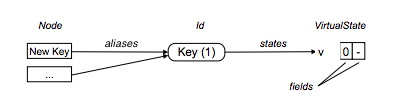
\includegraphics[width=0.9\textwidth]{DS-schema.png}
\caption{Schema of Basic Data Structures}
\label{figure-6}
\end{figure}

Αυτά τα αντικείμενα \textit{dictionaries} λέγονται \textit{state} γιατί
διατηρούν την κατάσταση των μεταβλητών για το εκάστοτε \texttt{Block}s που
βρίσκεται τώρα ο μεταγλωττιστής. Κάθε φορά που η επεξεργασία μετακινείται στο
επόμενο \texttt{Block} τότε δημιουργείται ένα αντίγραφο του \textit{state}.
Επιπλέον λεπτομέρειες για ποιό λόγο και πως συμβαίνει αυτό στο Κεφάλαιο 4.
Λοιπόν η πληροφορία για την κατάσταση των τρέχουσων μεταβλητών βρίσκεται σε αυτή
την δομή με μορφή αντικειμένων και όπως θα δούμε όταν υπάρχει ένα τέτοιο
αντικείμενο για μια μεταβλητή (συνδεόμενο φυσικά με αυτή με aliases και ids στο
\textit{state}) τότε το αντικείμενο είναι πάντα εικονικό. Αν δεν είναι εικονικό
το \texttt{VirtualObject} διαγράφεται από το \textit{state}, σε αντίθεση με την
μέθοδο που ακολουθείται στο paper. Εκεί προτείνεται η ύπαρξη δύο είδών εικονικών
αντικειμένων – ένα για την περίπτωση εικονικότητας (\texttt{VirtualState}) και
ένα για την περίπτωση αναγκαιότητάς του (\texttt{EscapedState}). Οι διαφορές
ήταν μικρές και κρίναμε ότι δεν ήταν αναγκαίο να υπάρχει κατάσταση και
αντικείμενο πληροφοριών για ένα αντικείμενο που υπάρχει στην μνήμη έτσι και
αλλίως αυτό καθ' αυτό.

Όπως βλέπουμε στο \ref{figure-6}, το πρώτο λευκό κουτάκι είναι το "node". Δηλαδή
μια αφαιρετική έννοια που περιλαμβάνει κυρίως ονόματα και references σε
μεταβλητές που υπήρχαν στην αρχική έκδοση του κώδικα. Αυτά "δείχνουν" στο id, το
οποίο είναι ουσιαστικά το όνομα που έχουμε δώσει στην μεταβλητή\footnote{ή
μεταβλητές} αυτή εσωτερικά – για δική μας χρήση μέσα στο σύστημά μας. Αυτό
δείχνει φυσικά στο εικονικό αντικείμενο που είναι μοναδικό για κάθε μεταβλητή
ανεξάρτητα από το πόσα ονόματα (aliases) έχει. Στην πραγματικότητα
χρησιμοποιούμε ένα \textit{defaultdict} της Python για να δείχνουμε κατευθείαν
απο τα nodes στα αντίστοιχα εικονικά αντικείμενα. Αυτό που φαίνεται στην εικόνα
είναι το θεωρητικό μοντέλο μας.

Να πούμε επίσης ότι στο paper εξηγείται πλήρως – και υπάρχει στο μοντέλο του – ο
τρόπος για το \textit{handling} όλων αυτών των διαδικασιών με δυνατότητες
κλειδώματος (locking) για παράλληλη επεξεργασία (βλ. \textit{multithreading}).
Εμείς δεν το συμπεριλαμβάνουμε αυτό, καθώς:

\begin{enumerate}

\item Δεν είναι αναγκαίο γιατί ασχολούμαστε με μεταγλωττιστές, ο εσωτερικός
κώδικας των οποίων δεν είναι συνήθως \textit{multi-threaded}.

\item Ακόμαι και αν χρειαστεί η δυνατότητα, η Python δεν το υποστηρίζει καλά
λόγω του καθολικού κλειδώματος που έχει (Global Interpreter Lock).

\end{enumerate}

%%%%%%%%%%%%%%%%%%%%%%%%%%%%%%%%%%%%%%%%%%%%%%%%%%%%%%%%%%%%%%%%%%%%%%

\subsubsection{Πότε αλλάζουν τα states}

Οι περιπτώσεις που επειρεάζονται τα state αντικείμενα – σύμφωνα πάντα με την
ιδανική κατάσταση του paper\cite{standler2014partial} και την υλοποίησή τους σε
Java (η οποία είναι ένας βελτιστοποιητής στον μεταγλωττιστή της που λέγεται
\textit{Graal}) – ή αλλιώς αυτά που χρήζουν προσοχής είναι:

\begin{itemize}

\item Κόμβοι (δηλαδή \texttt{Block}s) που περιέχουν εντολές δέσμευσης μνήμης
στον σωρό (malloc). Θα δημιουργήσουν εικονικά αντικείμενα.

\item Εντολές που κάποιο από τα argument τους περιέχουν keys σε υπάρχοντα
εικονικά αντικείμενα ή aliases σε αυτα. Οι εντολές τότε πρέπει να επεξεργαστούν
και είτε να μεταβληθούν είτε να αφαιρεθούν από τον κώδικα ολοκληρωτικά.

\item \texttt{Block}s που είναι ειδικά όπως \textit{mergeblock}
\textit{Returnblock} και \textit{LoopBegin}.

\end{itemize}

%%%%%%%%%%%%%%%%%%%%%%%%%%%%%%%%%%%%%%%%%%%%%%%%%%%%%%%%%%%%%%%%%%%%%%

\subsubsection{Πώς αλλάζουν τα states}

Θεωρητικά, σύμφωνα πάντα με το paper, αυτές οι αλλαγές στα states είναι οι
παρακάτω (τα γράμματα στις παρακάτω περιγραφές αντιστοιχούν στις εικόνες
\ref{figure-21} έως \ref{figure-24}):

\begin{enumerate}[label=\alph*]

\item Για κάθε δέσμευση, δημιουργούνται καινούργια εικονικά αντικείμενα \\
(\texttt{VirtualObject} – VOs) και τα αντίστοιχα entries στα mapping
dictionaries.

\begin{figure}[h]
\centering
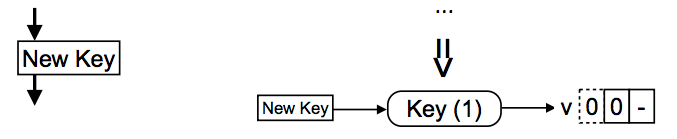
\includegraphics[width=0.5\textwidth]{virtual-alloc.png}
\caption{(ά) Actions upon allocation of a VO.}
\label{figure-21}
\end{figure}

\item Για κάθε "ανάθεση" (εντολή \texttt{setfield}) αντικειμένου που δεν είναι
σε κάποιο dictionary (states ή aliases – στην δική μας υλοποίηση: μόνο states)
σε πεδίο εικονικού αντικειμένου μεταβάλλεται η αντίστοιχη θέση μνήμης στο
attribute του εικονικού αντικειμένου ώστε αυτό να "ξέρει" περί της ανάθεσης. Το
γεγονός ότι το πρώτο αντικείμενο δεν ανήκε σε κάποιο dictionary μας δείχνει ότι
δεν είναι και αυτό εικονικό αντικείμενο, καθώς αν ήταν θα υπήρχε το alias του
στο dictionary. Αρα η παραπάνω περίπτωση είναι η περίπτωση ανάθεσης πραγματικού
– υπάρχοντος – αντικειμένου σε εικονικό.

\begin{figure}[h]
\centering
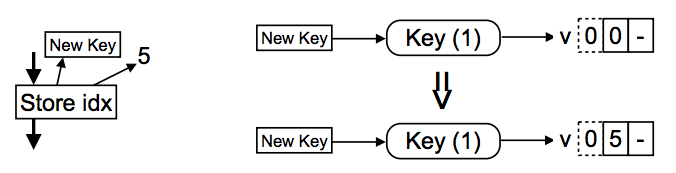
\includegraphics[width=0.5\textwidth]{virtual-ext-store.png}
\caption{(β') Actions upon simple external object storing inside a VO.}
\label{figure-22}
\end{figure}

\item Από την άλλη υπάρχει και η περίπτωση ανάθεσης εικονικού αντικειμένου σε
επίσης εικονικό αντικείμενου. Εδώ, θα αποθηκευτεί-ανατεθεί ένα
\textit{reference} του id του αντικειμένου που θα αποθηκευτεί, μέσα στο
αντικείμενο που αποθηκεύεται.

\begin{figure}[h]
\centering
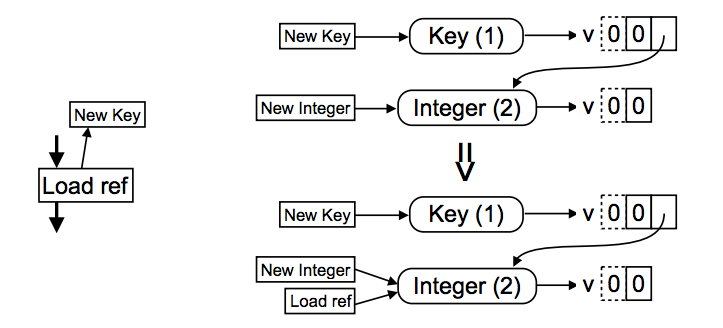
\includegraphics[width=0.5\textwidth]{virtual-virtual-load.png}
\caption{(γ') Actions upon assignment/loading of a VO inside another VO.}
\label{figure-23}
\end{figure}

\item Το παράνω φυσικά αναφέραται στην περίπτωση που θέλουμε να αποθηκέυσουμε
(store) το αντικείμενο. Στην αντίθετη, δηλαδή όταν θέλουμε να το ανακτήσουμε
μέσα από ένα άλλο που είναι επίσης εικονικό (με την εντολή \texttt{getfield}),
τότε η ανάγνωση αυτή θα οδηγήσει σε ανάθεση ενός καινούργιου alias έτσι ώστε ο
καινούργιος κώδικας, με τον οποίο θα αντικατασταθεί ο παλιός, να ξέρει που
υπάρχουν τώρα τα δεδομένα που χρειάζεται για την στιγμή που θα χρειαστεί να
γίνει το πραγματικό Load στο runtime.

\begin{figure}[h]
\centering
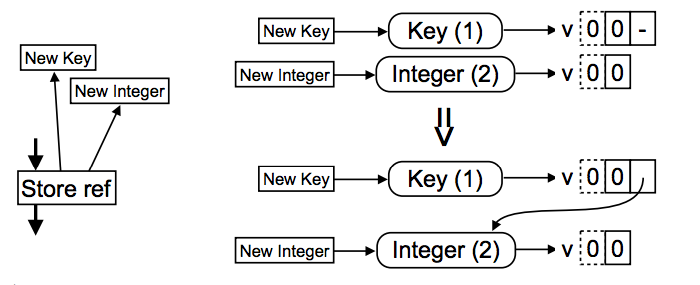
\includegraphics[width=0.5\textwidth]{virtual-virtual-store.png}
\caption{(δ') Actions upon storing a VO inside another VO.}
\label{figure-24}
\end{figure}

\end{enumerate}

Όλα αυτές οι εντολές θα αφαιρεθούν από τον κώδικα αφού, μόλις είπαμε οι
ενέργειες που λαμβάνει ο μεταγλωττιστής όταν τις συναντά αρκούν για να τις
κάνουν λειτουργικές και για τα side effects τους. Πολλές άλλες εντολές μπορούν
επίσης να αφαιρεθούν βάσει στις πληροφορίες που έχουμε στο states. Tests
ισότητας μεταξύ αντικειμένων επιστρέφουν πάντα \textit{false} αν ένα και μόνο
ένα από τα αντικείμενα που λάμβάνει το test είναι εικονικό. Εάν είναι και τα δύο
εικονικά, τότε θα παραχθεί \textit{true} αν φυσικά αναφέρονται στο ίδιο id, και
\textit{false} σε άλλη περίπτωση. (Αυτό το τσεκάρισμα, αργότερα στην υλοποίηση,
θα γίνεται κυρίως σε merge nodes όταν έχουμε αποφανθεί ότι το αντικείμενο θα
πρέπει να επανατοποθετηθεί στον κώδικα και θα θέλουμε να δοκιμάσουμε αν τα
αντικείμενα είναι ένα ή δυο.) Tests τύπων μπορούν να εκτελεστούν και σε αυτό το
σημείο (compile time). Αν κάποια εντολή που δεν είναι ειδική για αυτές τις
ενέργειες και δεν αναφέρεται εδώ απαιτεί ένα reference σε αντικείμενο το οποίο
είναι εικονικό τότε φυσικά αυτό θα πρέπει να επανατοποθετηθεί.

%%%%%%%%%%%%%%%%%%%%%%%%%%%%%%%%%%%%%%%%%%%%%%%%%%%%%%%%%%%%%%%%%%%%%%%%%%

\subsubsection{Ειδικές κατηγορίες: Merge}

Όταν πολλά branches της ροής θα συναντηθούν σε ένα \textit{mergenode}, πρέπει να
παράγουμε ένα state από όσα και τα branches. Αρχικά ο "επεξεργαστής" της
συγχώνευσης θα δημιουργήσει μια \textit{τομή} από όλα τα δεδομένα των
αντικειμένων state από όλα τα branches. Αυτό σημαίνει ότι τα εικονικά
αντικείμενα που θα επιβιώσουν την συγχώνευση είναι αυτά που είναι κοινά σε όλα
τα branches της ροής και έχουν τουλάχιστον έναν κοινό alias.

Οι περιπτώσεις που μπορούν να συμβούν ανάλογα με την κατάσταση των αντικειμένων
είναι οι εξής (σχεδιαγράμματα στις εικόνες \ref{figure-41} και \ref{figure-42}):

\begin{itemize}

\item Αν το αντικείμενο έχει διαφύγει σε όλες τις προηγούμενες καταστάσεις (τις
οποίες θέλουμε να συγχωνεύσουμε) τότε φυσικά το αντικείμενο θα διαφεύγει και στο
καινούργιο state.

\item Αν κάποια από τα αντικείμενα είναι εικονικά και άλλα διαφεύγουν, τότε
πρέπει να επανατοποθετηθούν και όσα αντικείμενα είναι εικονικά στα αντίστοιχα
states τους.

\item Η πιο ειδική περίπτωση είναι όλα τα αντικείμενα να είναι εικονικά. Τότε
στο καινούργιο αντικείμενο όλες οι τιμές από όλα τα states πρέπει να
συγχωνευτούν. Για κάθε field, ο μεταγλωττιστής θα κοιτάξει και θα συγκρίνει τις
εκδόσεις από όλα τα states και:

\begin{figure}[h]
\centering
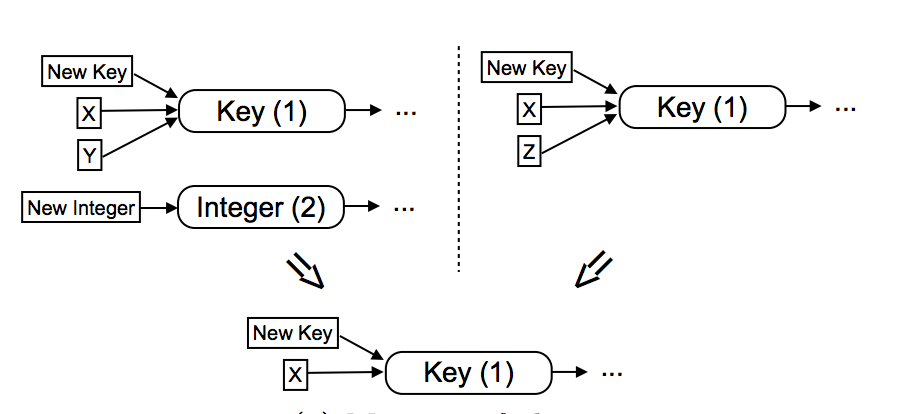
\includegraphics[width=0.5\textwidth]{merging-aliases.png}
\caption{Merging of aliases}
\label{figure-41}
\end{figure}

\begin{figure}[h]
\centering
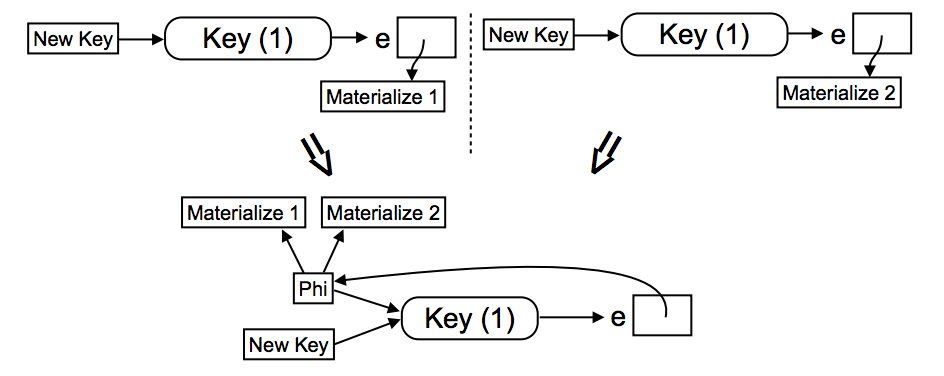
\includegraphics[width=0.5\textwidth]{merging-escaped.png}
\caption{Merging of escaped objects}
\label{figure-42}
\end{figure}

\begin{itemize}

\item αν όλα τα πεδία είναι πανομοιότυπα και συμφωνούν, τότε το καινούργιο
αντικείμενο στο συγχωνευμένο state μπορεί επίσης να είναι εικονικό. Ο
μεταγλωττιστής θα δημιουργήσει εδώ ένα καινούργιο \texttt{VirtualObject} και θα
αντιγράψει τα fields. Τα references θα δείχνουν στα ίδια ids κτλ.

\item αν κάποιο από τα πεδία διαφέρει το αντικείμενο πρέπει να επανατοποθετηθεί,
όπως επίσης και τα αντικείμενα για τα οποία περιέχει αναφορές.

\end{itemize}
\end{itemize}

Φυσικά αυτή η διαδικασία μπορεί να οδηγήσει στην επανατοποθέτηση αντικειμένων
που σημαίνει ότι προηγούμενες υποθέσεις που έχουν γίνει για τον κώδικα δεν είναι
πλέον αληθείς άρα θα πρέπει να γίνει επεξεργασία ξανά. Οπότε επαναλαμβάνουμε το
παραπάνω μέχρι να μην υπάρχουν αλλαγές.

%%%%%%%%%%%%%%%%%%%%%%%%%%%%%%%%%%%%%%%%%%%%%%%%%%%%%%%%%%%%%%%%%%%%%%%%%%

\subsubsection{Ειδικές κατηγορίες: Loops}

Οι βρόγχοι (loops) είναι μια πολύ ειδική περίπτωση. Όλοι οι κόμβοι
(\texttt{Block}s) που συμμετέχουν σε έναν βρόγχο πρεπεί και θα εξεταστούν με
σεριακό τρόπο ακολουθώντας την σειρά ροής, όμως αυτό ενέχει πρόβλημα με τις
"ακμές επιστροφής" (back edges) του βρόγχου. Φυσικά η κανονική ροή εδώ μπορεί να
επισκεφτεί κόμβους παραπάνω από μια φορά – αυτό είναι και το νόημα των loops –
αλλά εμείς δεν μπορούμε να το έχουμε αυτό κατα το compile time.

Η θεωρία που ακολουθείται στο paper, έχει φυσικά το παραπάνω χαρακτηριστικό αλλά
κρίναμε ότι είναι τουλάχιστον μη αποδοτική και δεν την υλοποιήσαμε στο δικό μας
σύστημα. Συνοπτικά να πούμε ότι ξεκινάει "μαντεύοντας" ένα state αντικείμενο (το
καλούν speculative) βάσει του κόμβου πατέρα του αρχικού κόμβου του βρόγχου και
από εκεί συνεχίζουν ακολουθώντας την ροή, σταματώντας μόνο στα back edges και
στα exits του loop. Το τελικό προϊόν είναι σωστό και η επεξεργασία συνεχίζεται
μόνο αν το αρχικο speculative state ήταν τελικά σωστό. Αν διαφέρουν, η
διαδικασία θα ξαναγίνει και το καινούργιο state θα χρησιμοποιηθεί ως speculative
state αυτή την φορά.

%%%%%%%%%%%%%%%%%%%%%%%%%%%%%%%%%%%%%%%%%%%%%%%%%%%%%%%%%%%%%%%%%%%%%%%%%%

\subsubsection{Πυροδότηση (triggering) \& σύνδεση με άλλους βελτιστοποιητές}

Στην θέση της μεταβλητής ή αντικειμένου που αφαιρέθηκε φυσικά θα πρέπει να
υπάρξει κάτι το οποίο "διατηρεί" την λογική του προγράμματος ως έχει. Αυτό
μπορεί να συμβεί με διάφορους τρόπους. Συνήθως επιτυγχάνεται με αντικατάσταση
βαθμωτών στην θέση της μεταβλητής. Δηλαδή το σημείο στο οποίο "ζητούνταν"
κάποιου είδους πληροφορία τοποθετείται ένας βαθμωτός, δηλαδή μια απλή "φθηνή"
μεταβλητή, που απλά υπάρχει στην στοίβα (\textit{function stack}) της συνάρτησης
και όχι στον σωρό (\textit{heap}). Σε αυτόν τον βαθμωτό ο μεταγλωττιστής
τοποθετεί την απαραίτητη πληροφορία που χρειάζεται το πρόγραμμα εκείνη την
στιγμή και κανονικά θα την εξήγαγε από το αντικείμενο που αφαιρέσαμε. Φυσικά την
πληροφορία αυτή ο μεταγλωττιστής την εξάγει επίσης από το αντικείμενο αλλά κατά
την ανάλυσή μας (στο \textit{compile-time}) και όχι στο \textit{runtime}. Ο
μεταγλωττιστής αποθηκεύει προσωρινά τις πληροφορίες που χρειάζεται για τυχόν
υπολογισμούς με τα αντικείμενα (για χρήση στο επόμενο σημείο που θα απαιτηθεί
βαθμωτός) στα εικονικά αντικείμενα που αναφέρουμε παραπάνω. Αν το αντικείμενο
πρέπει να επανατοποθετηθεί όλοι αυτοί οι βαθμωτοί θα αφαιρεθούν και οι ενέργειες
θα αναιρεθούν. Τέλος να πούμε ότι φυσικά πολλές από αυτές τις πράξεις θα
μεταφερθούν (\textit{carried on}) μέσω των εικονικών αντικειμένων και των
"προσωρινών" πράξεων και τα αποτελέσματά τους απλά θα τοποθετηθούν εκεί που
χρειάζονται "πραγματικά" – δηλαδή έξω από το scope της συνάρτησης που αναλύουμε.
Μπορεί κανείς να πει ότι αυτό είναι ένα είδος \textit{constant folding}.

Όλοι οι σύγχρονοι μεταγλωττιστές – συμπεριλαμβανομένου του PyPy – δουλεύουν με
κάποιου είδους εικονική μηχανή που αναλαμβάνει να τρέξει τον κώδικα και αυτές οι
μηχανές, εκτός απο πολλά πλεονεκτήματα ασφαλείας και ευκολίας προγραμματισμού,
έχουν φυσικά πολλούς τρόπυς βελτιστοποίησης του κώδικα, όπως έχουμε πει. Σε αυτά
περιλαμβάνεται και \textit{alias analysis} που εντοπίζει τα επιπλέον ονόματα των
μεταβλητών και σίγουρα μειώνει τον φόρτο εργασίας στην μνήμη. Επίσης
συμπεριλαμβάνεται πάντα ένας inliner (βλ. παραπάνω παράδειγμα). Η βελτιστοποίηση
με την μέθοδο μερικής διαφυγής λοιπόν είναι πολύ πιο αποδοτική από αυτά μόνη της
αλλά σίγουρα ακόμα περισσότερο όταν συνδυάζεται με επιπλέον βελτιστοποιήσεις και
τροποποιητές του κώδικα όπως το inlining.

Το \textit{inling} είναι η μεταφορά κομματιών κώδικα σε άλλα σημεία έτσι ώστε να
αποφευχθεί κάποια κλήση συνάρτησης. Ο μεταγλωττιστής φυσικά προβαίνει σε αυτό
όταν αποφανθεί ότι η κλήση αυτή καθ' αυτή – δηλαδή η δημιουργεία stack και ότι
άλλο περιλαμβάνει αυτό – είναι ακριβή και δεν αξίζει. Οπότε αντί για κλήση σε
συνάρτηση θα μεταφέρει τον κώδικα της συνάρτησης στο σημείο που βρίσκεται η ροή
την εκάστοτε στιγμή. Φυσικά πολλές φορές ο μεταγλωττιστής δεν θα το κάνει –
υπάρχει λόγος που πολλές φορές ο προγραμματιστής αποφασίζει να χρησιμοποιήσει
συναρτήσεις\footnote{εκτός από την ευκολότερη διαχείρηση του κώδικα} όταν π.χ. η
κλήση θα συμβεί πολλές φορές. Εαν προβούμε σε inlining σε αυτή την περίπτωση το
μέγεθος του κώδικα θα αυξηθεί δραματικά. Είναι προφανές ότι αυτού του είδους η
ενέργεια βοηθά το δικό μας έργο σε τεράστιο βαθμό. Οι μεταβλητές που
αποφασίζουμε ότι μπορούν να αφαιρεθούν είναι πολύ περισσότερες μετά το πέρασμα
του inliner, καθώς οποιαδήποτε μεταβλητή μπορεί να μεταφερθεί στην συνάρτηση
έχει μεταφερθεί. Ο inliner υλοποιείται στο αρχείο \texttt{inliner.py}.

Για επιπλέον πρακτικές λεπτομέρειες για το πως υλοποιήσαμε την παραπάνω θεωρία
και φυσικά ότι προβλήματα πραγματικού περιβάλλοντος συναντήσαμε κατά το
εγχείρημα αυτό βλ. επόμενο κεφάλαιο.

%------------------------------------------------------------------------------

\subsection{Παράδειγμα}

Εδώ παραθέσουμε ένα εκτενές παράδειγμα, αυτή τη φορά φυσικά για τις διαφορές και
λεπτομέρειες της μερικής ανάλυσης με περισσότερη \textit{real-world} λεπτομέρεια
από το αντίστοιχο της απλής ανάλυσης, ακολουθώντας φυσικά το παράδειγμα του
paper\cite{stadler2014partial} εξιδανικευμένο για την Python. Αυτή την φορά ο
αρχικός κώδικας είναι μετά το inlining για να αναδείξουμε καλύτερα τα
αποτελέσματα της ανάλυσης διαφυγής.

\begin{lstlisting}[language=Python]
...
def getValue(idx, ref):
    key = Key()
    key.idx = idx
    key.ref = ref
    tmp1 = cacheKey # getting from a global
    tmp2 = (key.idx == tmp1.idx && key.ref == tmp1.ref)
    if tmp2:
        return cacheValue
    else:
        cacheKey = key # assigning to a global
        cacheValue = createValue(...)
        return cacheValue
...
\end{lstlisting}

Ξανά δεν δίνουμε τις καθολικές (global) μεταβλητές (βλ. γραμμή 5) και πολλές
λεπτομέρειες που θα επιβάρυναν τον κώδικα χωρίς να προσφέρουν επιπλέον
πληροφορία. Αναδεικνύουμε παρακάτω πως θα ήταν σε κώδικα Python η
βελτιστοποιημένη έκδοση του παραπάνω κώδικα. Επαναλαμβάνουμε ότι αυτή η
λειτουργία γίνεται σε γραφήματα ροής.

\begin{lstlisting}[language=Python]
...
def getValue(idx, ref):
    tmp = cacheKey
    if (key.idx == tmp.idx && key.ref == tmp.ref):
        return cacheValue
    else:
        key = Key()
        key.idx = idx
        key.ref = ref
        cacheKey = key
        cacheValue = createValue(...)
        return cacheValue
...
\end{lstlisting}

Βλέπουμε τον τρόπο που ο βελτιστοποιητής άλλαξε τον κώδικάς μας.

\begin{itemize}

\item Στην γραμμή 3 η δέσμευση (η δημιουργία ουσιαστικά του αντικειμένου) έχει
αφαιρεθεί. Δημιουργείται εικονικό αντικείμενο.\footnote{Για περισσότερες
λεπτομέρειες για τα εικονικά αντικείμενα βλ. προηγούμενο κεφάλαιο}

\item Οι αναθέσεις στις γραμμές 4 και 5 έχουν επίσης αφαιρεθεί. Γίνεται
"ανάκλαση" των αποτελεσμάτων τους και των side-effect τους στα εικονικά
αντικείμενα.

\item Οι απόπειρες πρόσβασης σε περιοχές δεσμευμένης μνήμης στην γραμμή 7 έχουν
αντικατασταθεί με απλές προσβάσεις σε τοπικές περιοχές.

\item Στην περίπτωση του \texttt{if} στην γραμμή 8, δημιουργείται ένα επιπλέον
αντίγραφο της δομής δεδομένων που διαχειρίζεται τα εικονικά αντικείμενα
(\textit{state} – βλ. παρακάτω).

\item Στην γραμμή 9 το αντικείμενο είναι ακόμα εικονικό. Λόγω της εντολής
\texttt{return} η διαδικασία ανάλυσης αυτού του branch (του if) τερματίζει εδώ.

\item Η ανάλυση για το δεύτερο branch όμως συνεχίζεται στο \textit{else case}
εδώ. Στην στιγμή της γραμμή 11 το αντικείμενο είναι ακόμα εικονικό όμως λόγω της
ανάθεσης σε καθολική μεταβλητή θα "διαφύγει". Για να μπορεί να γίνει αυτό όμως,
το αντικείμενο θα πρέπει να υπάρχει αυτό καθ' αυτό, οπότε θα πρέπει να
τοποθετηθεί στον κώδικα η δέσμευση της μνήμης, η αρχικοποίησή της, η ανάθεση των
field σύμφωνα με το εικονικό αντικείμενο (και ότι άλλο υπεισέρχεται στην
δημιουργία ενός αντικειμένου). Ονομάζουμε αυτή την διαδικασία
\textit{materialization} (βλ. επόμενο κεφάλαιο).

\item Οι γραμμές 12 και 13 δεν επηρεάζουν πλέον την κατάσταση του κώδικα – αφού
έχουμε ήδη αποφανθεί ότι το αντικείμενο πρέπει να υπάρχει.

\end{itemize}

Γενικά, όπως βλέπουμε, η δέσμευση και όλες οι ακριβές ενέργειες έχουν
τοποθετηθεί ακριβώς εκεί που απαιτούνται και όχι οπουδήποτε αλλού – δηλαδή στο
\textit{else case} του \textit{if branch}. Αυτό προφανώς δεν οδηγεί σε μικρότερο
αριθμό εντολών \texttt{malloc} (ούτε άλλων ακριβών εντολών) αλλά μειώνει τον
δυναμικό αριθμό των δεσμεύσεων μνήμης αφού αυτοί θα συμβούν πιο σπάνια δεδομένου
ότι βρίσκονται σε ένα από τα \textit{cases} και όχι στην κυρίως ροή του κώδικα.
Με άλλα λόγια μειώνουν το μέσο κόστος της συνάρτησης, βασιζόμενοι στην μικρότερη
συχνότητα με την οποία τρέχουν τα \textit{branches}. Όπως θα δούμε στο κεφάλαιο
των μετρήσεων (Κεφ. 5.) αυτό συμβαίνει συχνά.
